\documentclass[uplatex,dvipdfmx]{beamer}
\usepackage{listings,jvlisting}
\usepackage{color}
\usepackage{xr}

\lstset{
  backgroundcolor=\color[rgb]{0.9,0.9,0.9},
  frame=single,
  basicstyle=\ttfamily
}
\makeatletter
\newcommand*{\addFileDependency}[1]{% argument=file name and extension
  \typeout{(#1)}
  \@addtofilelist{#1}
  \IfFileExists{#1}{}{\typeout{No file #1.}}
}
\makeatother

\newcommand*{\myexternaldocument}[1]{%
    \externaldocument{#1}%
    \addFileDependency{#1.tex}%
    \addFileDependency{#1.aux}%
}
\myexternaldocument{../categoryTheoryIntro/CategoryTheoryIntro}

\newcommand{\pr}[1]{\colorbox[rgb]{0.9,0.9,0.9}{\lstinline{#1}}}
\newcommand{\functype}[2]{\pr{#1 -> #2}}
\newcommand{\refcti}[1]{\cite{cti}\ref{#1}}
\newcommand{\fpmor}[3]{\pr{#1 :: #2 -> #3}}
\usefonttheme[onlymath]{serif}

\usepackage{tikz}
\usepackage{bbm}
\usepackage{amsmath,amssymb}
\usepackage{url}
\usetikzlibrary{matrix,arrows}

\newcommand{\cat}[1]{\mathbbm{#1}}
\newcommand{\arrow}{\rightarrow}
\newcommand{\functor}[3]{#1:\cat{#2}\arrow \cat{#3}}
\newcommand{\profunctor}[3]{#1:\cat{#2}\nrightarrow \cat{#3}}

\newcommand{\nat}[3]{#1:#2\Rightarrow #3}
\newcommand{\natf}[5]{#1:#2\Rightarrow #3:\cat{#4}\arrow \cat{#5}}
\newcommand{\tuple}[1]{\langle #1\rangle}
\newcommand{\objr}[1]{\mathrm{Obj}(#1)}
\newcommand{\obj}[1]{\mathrm{Obj}(\cat{#1})}
\newcommand{\morset}[1]{\mathrm{Mor}(\cat{#1})}

\newcommand{\mor}[3]{#1:#2\arrow #3}
\newcommand{\dom}{\mathrm{dom}}
\newcommand{\cod}{\mathrm{cod}}
\newcommand{\arset}[3]{\cat{#1}(#2,#3)}
\newcommand{\arsetr}[3]{#1(#2,#3)}
\newcommand{\pcobj}[1]{[#1]}
\newcommand{\funccat}[2]{\cat{#2}^\cat{#1}}

\newcommand{\coend}[2]{\displaystyle\int^{#2:\cat{#1}}\!\!\!\!\!\!\!}
\newcommand{\cend}[2]{\displaystyle\int_{#2:\cat{#1}}\!\!\!\!\!\!\!}
\newcommand{\natlat}[3]{\{#1\}_{#3\in #2}}
\newcommand{\inset}[2]{[#1,#2]}
\newcommand{\incat}[2]{[\cat{#1},\cat{#2}]}
\newcommand{\incatp}[2]{[#1,#2]}

\newenvironment{mydescription}
{\begin{description}
  \setlength{\parskip}{0.5cm}
}
{\end{description}}
\title{プロファンクターオプティクスの理論と実装}
\author{\input{../myname}}
\usetheme{Madrid}
\setbeamertemplate{navigation symbols}{}
\begin{document}
  \begin{frame}
    \titlepage
  \end{frame}
  \begin{frame}\frametitle{目的}
    データへのアクセサの一般化であるLensやキャストの一般化であるPrismは更にOpticsという概念へと一般化される。\\
    これらの一般化には圏論が用いられるが、圏論は自身を抽象化できることが多く。Opticsに関する議論を更に高度な圏論で一般化できると考えた。\\
    \vspace{\baselineskip}
    特に圏同値\[\cat{Tamb}\simeq\incat{Optic}{Set}\]の圏論的一般化を試みた。
  \end{frame}
  \begin{frame}\frametitle{表記について}
    今回は圏論の具体例として集合の操作を中心に用いる。これは以下のようにプログラムと対応するため適宜読み替えてほしい。また時間の都合上厳密な議論は省略する。
    \begin{table}[h]
      \centering
      \begin{tabular}{|c|c|c|c|c|c|c|}
        \hline
        集合&集合&写像&要素\\
              &$A$ &$\mor{f}{A}{B}$&$a\in A$\\
        \hline
    プログラム&型  &関数&値\\
              (Haskell)&\pr{a}&\pr{f :: a -> b}&\pr{x :: a}\\
        \hline
      \end{tabular}
    \end{table}
    また集合$A,B$の直積集合、直和集合を$A\times B$、$A+B$とし、\\
    集合$A$を集合$B$へ写す写像の集合を$\inset{A}{B}$とする。
  \end{frame}
  \begin{frame}\frametitle{データアクセサの一般化Lens}
    \begin{definition}[Lens]
      Lensは以下の二つの写像で構成される。
      \[\mor{\mathrm{get}}{S}{A},\ \mor{\mathrm{set}}{S\times A'}{S'}\]
    \end{definition}
    ここで$S:=B\times A,\ S':=B\times A'$とすると、
    \begin{alignat*}{7}
      \mathrm{get}:\ &S\ &\longrightarrow \ &A \ \ \ &\mathrm{set}:\ &S\times A'\ &\longrightarrow \ &S'\\
      &\tuple{b,a}&\longmapsto\ &a      &&\tuple{\tuple{b,a},a'}&\longmapsto\ &\tuple{b, a'}
    \end{alignat*}
    またこのような二つの写像の組の全体を$\mathrm{Lens}(A,A',S,S')$とする。すなわち\[\mathrm{Lens}(A,A',S,S') := \inset{S}{A}\times \inset{S\times A'}{S'}\]となる。
  \end{frame}
  \begin{frame}\frametitle{キャストの一般化Prism}
    \begin{definition}[Prism]
      Prismは以下の二つの射で構成される。
      \[\mor{\mathrm{down}}{S}{S' + A},\ \mor{\mathrm{up}}{A'}{S'}\]
    \end{definition}
    ここで$S:=B+ A,\ S':=B+ A'$とすると、
    \begin{alignat*}{20}
      \mathrm{down}:\ &S\ \ &\longrightarrow \ \ &S'+&A & \ \ \ \ \mathrm{up}: &A'&\longrightarrow &\ S'\\
      &a \ \ &\longmapsto \ \ &&a &&a'&\longmapsto &a'\\
      &b \ \ &\longmapsto \ \ &b& &
    \end{alignat*}
    Lensと同様に\[\mathrm{Prism}(A,A',S,S') := \inset{S}{S'+A}\times\inset{A'}{S}\]とする。
  \end{frame}
  \begin{frame}\frametitle{LensとPrismの双対性}
    \begin{theorem}
     LensとPrismは双対である。
    \end{theorem}
    \vspace{\baselineskip}
    二つの概念が双対であるとは、それを構成する射の向きがすべて逆であることである。例えば積と余積はどちらも以下の図式によって定義される。
    {\tiny
    \begin{center}
      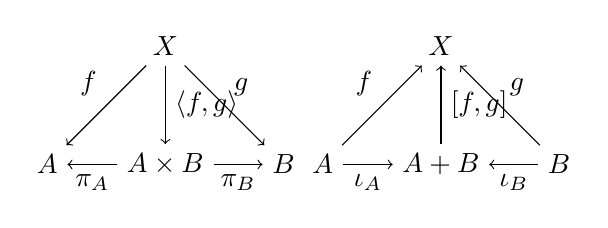
\begin{tikzpicture}[auto]
        \node (X) at (0, 1.5) {$X$};
        \node (AB) at (0, 0) {$A\times B$};
        \node (A) at (-1.5, 0) {$A$};
        \node (B) at (1.5, 0) {$B$};

        \draw[->] (X) to node[swap]{$f$}(A);
        \draw[->] (X) to node{$g$}(B);
        \draw[->] (AB) to node{$\pi_A$}(A);
        \draw[->] (AB) to node[swap]{$\pi_B$}(B);
        \draw[->] (X) to node{$\tuple{f,g}$}(AB);

        \node (X) at (3.5, 1.5) {$X$};
        \node (AB) at (3.5, 0) {$A+B$};
        \node (A) at (2, 0) {$A$};
        \node (B) at (5, 0) {$B$};

        \draw[<-] (X) to node[swap]{$f$}(A);
        \draw[<-] (X) to node{$g$}(B);
        \draw[<-] (AB) to node{$\iota_A$}(A);
        \draw[<-] (AB) to node[swap]{$\iota_B$}(B);
        \draw[<-] (X) to node{$[f,g]$}(AB);
      \end{tikzpicture}
    \end{center}}
    これによってLens\ $\inset{S}{A}\times \inset{S\times A'}{S'}$とPrism\ $\inset{S}{S'+A}\times\inset{A'}{S}$が双対の関係にあると分かる。
  \end{frame}
  \begin{frame}\frametitle{Opticの定義}
    \begin{definition}[Optic]
      四つの集合$A,A',S,S'$に対するOpticの集合を\[\mathrm{Optic}(A,A',S,S') := \int^M \inset{S}{M\otimes A}\times \inset{M\otimes A'}{S'}\]と定義する。
    \end{definition}
    ただしこの定義に出てくる以下の二つの概念は個別に詳しく説明する。\\
    \vspace{\baselineskip}

    \begin{mydescription}
      \item[モノイダル積$\otimes$] 直積$\times$、直和$+$の一般化
      \item[コエンド$\int^M$] 集合で添字付けられた直和集合を取り、ある同値関係で割る操作
    \end{mydescription}
  \end{frame}
  \begin{frame}\frametitle{モノイダル積}
    集合を要素として定義される二項演算$\otimes$がモノイダル積である時以下の性質を満たす。\\
    \vspace{\baselineskip}

    \begin{mydescription}
      \item[結合則] $(A\otimes B)\otimes C$と$A\otimes(B\otimes C)$が一対一対応
      \item[単位則] ある集合$I$が存在し、$A\otimes I$と$A$が一対一対応\\
      直積の場合の$I$は単集合であり、直和の場合は空集合である。
      \item[並列性] 集合のみならず、二つの写像$\mor{f}{A}{B},\ \mor{g}{C}{D}$を合成した写像
      \[\mor{f\otimes g}{A\otimes C}{B\otimes D}\]が得られる。
    \end{mydescription}
  \end{frame}
  \begin{frame}\frametitle{コエンド}
    $\int^M \inset{S}{M\otimes A}\times \inset{M\otimes A'}{S'}$の任意の要素はある集合$M$に対して$\mor{l}{S}{M\otimes A},\ \mor{r}{M\otimes A'}{S}$となるような写像の組$\tuple{l,r}$である。\\
    \vspace{\baselineskip}
    ただし写像$\mor{l}{S}{M\otimes A},\mor{r}{N\otimes A'}{S'},\ \mor{f}{M}{N}$に対して\[\tuple{(f\otimes A)\circ l,r} = \tuple{l,r\circ (f\otimes A')}\]が成り立つ。
    {\scriptsize
    \begin{center}
      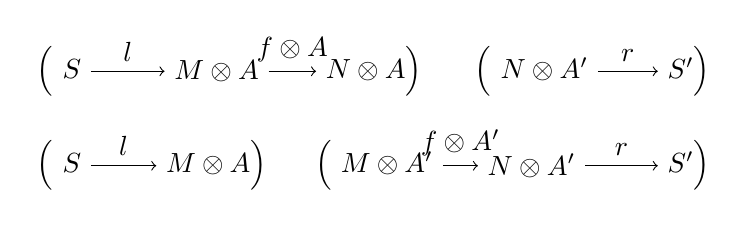
\begin{tikzpicture}[auto]
        \node (S) at (0, 0) {\Big( $S$};
        \node (MA) at (2, 0) {$M\otimes A$};
        \node (NA) at (4, 0) {$N\otimes A$\Big)};
        \node (NA') at (6, 0) {\Big( $N\otimes A'$};
        \node (S') at (8, 0) {$S'$\Big)};
        \draw[->] (S) to node{$l$}(MA);
        \draw[->] (MA) to node{$f\otimes A$}(NA);
        \draw[->] (NA') to node{$r$}(S');

        \node (S) at (0, -1.2) {\Big( $S$};
        \node (MA) at (2, -1.2) {$M\otimes A$\Big)};
        \node (MA') at (4, -1.2) {\Big( $M\otimes A'$};
        \node (NA') at (6, -1.2) {$N\otimes A'$};
        \node (S') at (8, -1.2) {$S'$\Big)};
        \draw[->] (S) to node{$l$}(MA);
        \draw[->] (MA') to node{$f\otimes A'$}(NA');
        \draw[->] (NA') to node{$r$}(S');
      \end{tikzpicture}
    \end{center}}
  \end{frame}
  \begin{frame}\frametitle{ストリングダイアグラム}
    モノイダル積の並列性$\mor{f\otimes g}{A\otimes C}{B\otimes D}$を以下のように表す。
    \begin{center}
      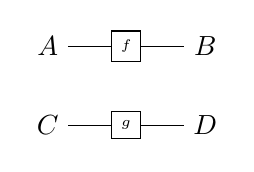
\begin{tikzpicture}
        \node (A) at (0, 0) {$A$};
        \node (B) at (2, 0) {$B$};
        \node (C) at (0, -1) {$C$};
        \node (D) at (2, -1) {$D$};
        \draw[-] (A) to node[draw, fill=white]{\tiny{$f$}}(B);
        \draw[-] (C) to node[draw, fill=white]{\tiny{$g$}}(D);
      \end{tikzpicture}
    \end{center}
    すると$\int^M \inset{S}{M\otimes A}\times \inset{M\otimes A'}{S'}$のある要素$\tuple{l,r}$は
    \begin{center}
      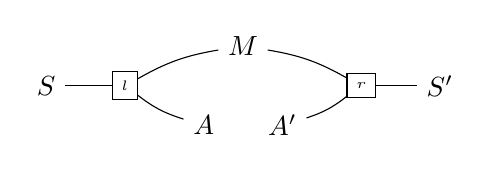
\begin{tikzpicture}
        \node (S) at (0, 0) {$S$};
        \node (M) at (2.5, 0.5) {$M$};
        \node (A) at (2, -0.5) {$A$};

        \node[draw] (l) at (1, 0) {{\tiny$l$}};
        \draw[-] (S) to (l);
        \draw[-] (l) to [bend left=10] (M);
        \draw[-] (l) to [bend right=10](A);

        \node (S') at (5, 0) {$S'$};
        \node (A') at (3, -0.5) {$A'$};
        \node[draw] (r) at (4, 0) {{\tiny$r$}};
        \draw[-] (r) to (S');
        \draw[-] (r) to [bend right=10] (M);
        \draw[-] (r) to [bend left=10](A');
      \end{tikzpicture}
    \end{center}
    と書くことができる。また$l,r$から伸びる$M$についてはコエンドの性質により線を繋げるのが妥当である。
  \end{frame}
  \begin{frame}
    \frametitle{LensはOpticである}
    モノイダル積$\otimes$が直積$\times$である時、
    \begin{center}
      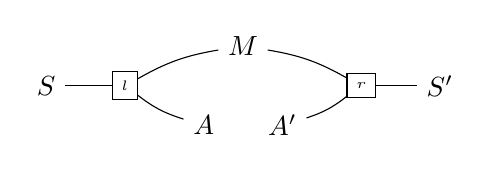
\begin{tikzpicture}
        \node (S) at (0, 0) {$S$};
        \node (M) at (2.5, 0.5) {$M$};
        \node (A) at (2, -0.5) {$A$};

        \node[draw] (l) at (1, 0) {{\tiny$l$}};
        \draw[-] (S) to (l);
        \draw[-] (l) to [bend left=10] (M);
        \draw[-] (l) to [bend right=10](A);

        \node (S') at (5, 0) {$S'$};
        \node (A') at (3, -0.5) {$A'$};
        \node[draw] (r) at (4, 0) {{\tiny$r$}};
        \draw[-] (r) to (S');
        \draw[-] (r) to [bend right=10] (M);
        \draw[-] (r) to [bend left=10](A');
      \end{tikzpicture}
    \end{center}
    Hom関手の連続性$\inset{A}{B\times C}\cong\inset{A}{B}\times \inset{A}{C}$より、
    \begin{center}
      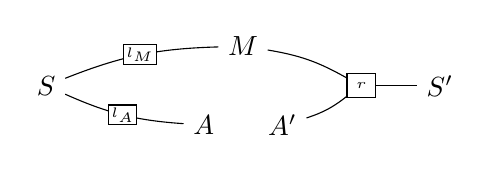
\begin{tikzpicture}
        \node (S) at (0, 0) {$S$};
        \node (M) at (2.5, 0.5) {$M$};
        \node (A) at (2, -0.5) {$A$};

        \draw[-] (S) to [bend left=10] node [draw,inner sep=1pt, fill=white]{\tiny$l_M$} (M);
        \draw[-] (S) to [bend right=10]node [draw,inner sep=1pt, fill=white]{\tiny$l_A$}(A);

        \node (S') at (5, 0) {$S'$};
        \node (A') at (3, -0.5) {$A'$};
        \node[draw] (r) at (4, 0) {{\tiny$r$}};
        \draw[-] (r) to (S');
        \draw[-] (r) to [bend right=10] (M);
        \draw[-] (r) to [bend left=10](A');
      \end{tikzpicture}
    \end{center}
    となり、余米田の補題$FA\cong\int^M [A,M]\times FM$から
    \begin{center}
      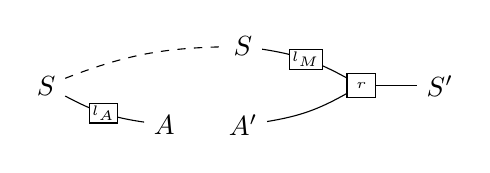
\begin{tikzpicture}
        \node (S) at (0, 0) {$S$};
        \node (A) at (1.5, -0.5) {$A$};
        \node (S2) at (2.5, 0.5) {$S$};
        \draw[-,dashed] (S) to [bend left=10] (S2);


        \draw[-] (S) to [bend right=10]node [draw,inner sep=1pt, fill=white]{\tiny$l_A$}(A);

        \node (S') at (5, 0) {$S'$};
        \node (A') at (2.5, -0.5) {$A'$};
        \node[draw] (r) at (4, 0) {{\tiny$r$}};
        \draw[-] (r) to (S');
        \draw[-] (r) to [bend right=10]node [draw,inner sep=1pt, fill=white]{\tiny$l_M$} (S2);
        \draw[-] (r) to [bend left=10](A');

      \end{tikzpicture}
    \end{center}
    よって$\mathrm{Optics}_\times(A,A',S,S') \cong \mathrm{Lens}(A,A',S,S')$
  \end{frame}
  \begin{frame}
    \frametitle{PrismはOpticである}
    モノイダル積$\otimes$が直和$+$である時、
    \begin{center}
      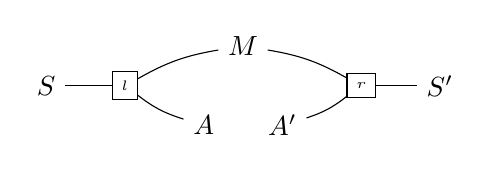
\begin{tikzpicture}
        \node (S) at (0, 0) {$S$};
        \node (M) at (2.5, 0.5) {$M$};
        \node (A) at (2, -0.5) {$A$};

        \node[draw] (l) at (1, 0) {{\tiny$l$}};
        \draw[-] (S) to (l);
        \draw[-] (l) to [bend left=10] (M);
        \draw[-] (l) to [bend right=10](A);

        \node (S') at (5, 0) {$S'$};
        \node (A') at (3, -0.5) {$A'$};
        \node[draw] (r) at (4, 0) {{\tiny$r$}};
        \draw[-] (r) to (S');
        \draw[-] (r) to [bend right=10] (M);
        \draw[-] (r) to [bend left=10](A');
      \end{tikzpicture}
    \end{center}
    反変Hom関手の余連続性$\inset{A+B}{C}\cong\inset{A}{C}+\inset{B}{C}$より、
    \begin{center}
      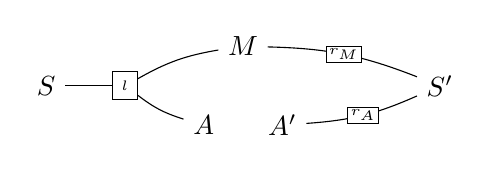
\begin{tikzpicture}
        \node (S) at (0, 0) {$S$};
        \node (M) at (2.5, 0.5) {$M$};
        \node (A) at (2, -0.5) {$A$};
        \node[draw] (l) at (1, 0) {{\tiny$l$}};
        \draw[-] (S) to (l);
        \draw[-] (l) to [bend left=10] (M);
        \draw[-] (l) to [bend right=10](A);

        \node (S') at (5, 0) {$S'$};
        \node (A') at (3, -0.5) {$A'$};
        \draw[-] (S') to [bend right=10] node [draw,inner sep=1pt, fill=white]{\tiny$r_M$} (M);
        \draw[-] (S') to [bend left=10]node [draw,inner sep=1pt, fill=white]{\tiny$r_A$}(A');
      \end{tikzpicture}
    \end{center}
    となり、余米田の補題$FA\cong\int^M [M,A]\times FM$から
    \begin{center}
      \begin{tikzpicture}
        \node (S) at (0, 0) {$S$};
        \node (M) at (2.5, 0.5) {$S'$};
        \node (A) at (2.5, -0.5) {$A$};
        \node[draw] (l) at (1, 0) {{\tiny$l$}};
        \draw[-,dashed] (S') to [bend right=10] (M);

        \draw[-] (S) to (l);
        \draw[-] (l) to [bend left=10] (M);
        \draw[-] (l) to [bend right=10](A);

        \node (S') at (5, 0) {$S'$};
        \node (A') at (3.5, -0.5) {$A'$};
        \draw[-] (M) to [bend right=10] node [draw,inner sep=1pt, fill=white]{\tiny$r_M$} (l);
        \draw[-] (S') to [bend left=10]node [draw,inner sep=1pt, fill=white]{\tiny$r_A$}(A');
      \end{tikzpicture}
    \end{center}
    よって$\mathrm{Optics}_\times(A,A',S,S') \cong \mathrm{Prism}(A,A',S,S')$
  \end{frame}
  \begin{frame}
    \frametitle{集合の圏}
    集合と写像の全体は圏と呼ばれる構造を持ち、これを$\cat{Set}$とする。\\
    \vspace{\baselineskip}
    \begin{definition}[集合の圏]
      {\small
      \begin{description}
        \item[対象] 任意の(小さい)集合を$\cat{Set}$の対象とする。
        \item[射] 対象$A,B$に対する射を任意の写像$\mor{f}{A}{B}$とする。
        \item[射の合成] 射の合成$f\circ g$はそのまま写像の合成とする。
      \end{description}
    }
    \end{definition}
  \vspace{\baselineskip}

  写像の集合は$\inset{A}{B}$で表せるが、これをOpticの集合$\mathrm{Optic}(A,A',S,S')$と置くと同様に圏が定義できる。
  \end{frame}
  \begin{frame}
    \frametitle{Opticの圏}
    \begin{definition}[Opticの圏]
      集合の圏上のOpticの圏を以下のように構成する。
      {\small
      \begin{description}
        \item[対象] 任意の(小さい)集合のニつ組を対象とする。
        \item[射] 対象$(A,A'),\ (S,S')$による射集合を$\mathrm{Optic}(A,A',S,S')$とする。
        \item[射の合成] 二つのOptic $\tuple{l',r'},\ \tuple{l,r}$の合成を$\tuple{(N\otimes l)\circ l',r'\circ(N\otimes r')}$とする。
      \end{description}
    }
    \end{definition}
    \begin{center}
      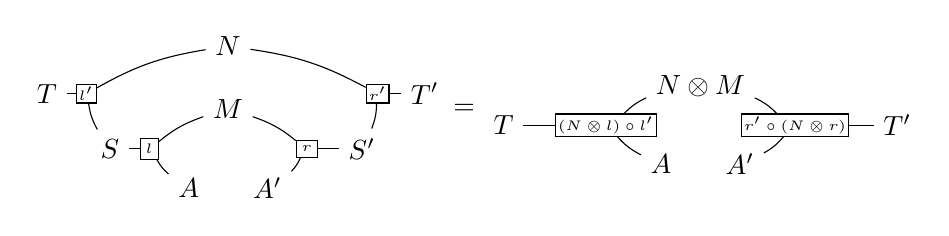
\begin{tikzpicture}
        \node (T) at (-0.8, 0.7) {$T$};

        \node (S) at (0, 0) {$S$};
        \node (M) at (1.5, 0.5) {$M$};
        \node (A) at (1, -0.5) {$A$};
        \node (N) at (1.5, 1.3) {$N$};

        \node[draw,inner sep=2pt] (l) at (0.5, 0) {{\tiny$l$}};

        \draw[-] (S) to (l);
        \draw[-] (l) to [bend left=10] (M);
        \draw[-] (l) to [bend right=10](A);
        \node[draw,inner sep=1pt] (l') at (-0.3, 0.7) {{\tiny$l'$}};
        \draw[-] (T) to (l');
        \draw[-] (l') to [bend right=10](S);
        \draw[-] (l') to [bend left=10] (N);

        \node (T') at (4, 0.7) {$T'$};
        \node (S') at (3.2, 0) {$S'$};
        \node (A') at (2, -0.5) {$A'$};
        \node[draw,inner sep=2pt] (r) at (2.5, 0) {{\tiny$r$}};
        \draw[-] (r) to (S');
        \draw[-] (r) to [bend right=10] (M);
        \draw[-] (r) to [bend left=10](A');

        \node[draw,inner sep=1pt] (r') at (3.4, 0.7) {{\tiny$r'$}};
        \draw[-] (T') to (r');
        \draw[-] (r') to[bend left=10] (S');
        \draw[-] (r') to [bend right=10] (N);

        \node (eq) at (4.5, 0.5) {$=$};

        \node (S) at (5, 0.3) {$T$};
        \node (M) at (7.5, 0.8) {$N\otimes M$};
        \node (A) at (7, -0.2) {$A$};

        \node[draw,inner sep=1pt] (l) at (6.3, 0.3) {{\tiny$(N\otimes l)\circ l'$}};
        \draw[-] (S) to (l);
        \draw[-] (l) to [bend left=10] (M);
        \draw[-] (l) to [bend right=10](A);

        \node (S') at (10, 0.3) {$T'$};
        \node (A') at (8, -0.2) {$A'$};
        \node[draw,inner sep=1pt] (r) at (8.7, 0.3) {{\tiny$r'\circ(N\otimes r)$}};
        \draw[-] (r) to (S');
        \draw[-] (r) to [bend right=10] (M);
        \draw[-] (r) to [bend left=10](A');
      \end{tikzpicture}
      \begin{tikzpicture}

      \end{tikzpicture}
    \end{center}
    またOpticの合成が定義できるので、Lens、Prismでも合成ができる。
  \end{frame}
  \begin{frame}
    \frametitle{丹原加群}

      \begin{definition}[丹原加群]
        丹原加群とは以下の図式を可換にするプロファンクター$P$と射の族\[\mor{\zeta_{A,A',M}}{P(A,A')}{P(M\otimes A, M\otimes A')}\]の組$(P,\zeta)$である。
      {\tiny
      \begin{center}
        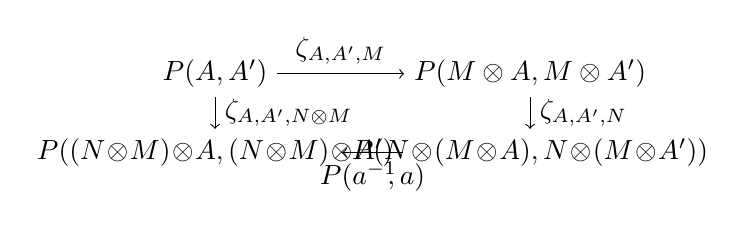
\begin{tikzpicture}[auto]
          \node (P) at (0, 0) {$P(A,A')$};
          \node (TP) at (4, 0) {$P(M\otimes A,M\otimes A')$};
          \node (TP2) at (0, -1) {$P((N\!\otimes\!M)\!\otimes\!A,(N\!\otimes\! M)\!\otimes\! A')$};
          \node (TTP) at (4, -1) {$P(N\!\otimes\! (M\!\otimes\! A),N\!\otimes\! (M\!\otimes\! A'))$};
          \draw[->] (P) to node{$\zeta_{A,A',M}$}(TP);
          \draw[->] (P) to node{$\zeta_{A,A',N\otimes M}$}(TP2);
          \draw[->] (TP) to node{$\zeta_{A,A',N}$}(TTP);
          \draw[->] (TP2) to node{$P(a^{-1}\!\!,a)$}(TTP);
        \end{tikzpicture}
        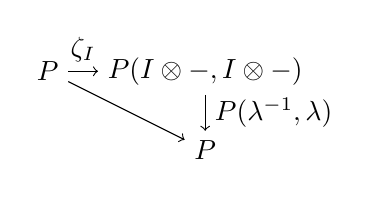
\begin{tikzpicture}[auto]
          \node (P) at (0, 0) {$P$};
          \node (TP) at (2, 0) {$P(I\otimes -,I\otimes -)$};
          \node (P2) at (2, -1) {$P$};
          \draw[->] (P) to node{$\zeta_I$}(TP);
          \draw[->] (TP) to node{$P(\lambda^{-1},\lambda)$}(P2);
          \draw[->] (P) to(P2);
        \end{tikzpicture}
      \end{center}}
      \end{definition}
      ただし、プロファンクターとは圏上の二項演算であって、二つの射$\mor{f}{B}{A},\ \mor{g}{C}{D}$に対して$\mor{P(f,g)}{P(A,C)}{P(B,D)}$が得られる。\\
      ただし、モノイダル積とは射$f$の向きが異なることに注意\\
  \end{frame}
  \begin{frame}
    \frametitle{丹原加群の圏}
    \begin{definition}[丹原加群の圏]
      丹原加群の圏$\cat{Tamb}$を以下のように定義する。
      {\small
      \begin{description}
        \item[対象] 任意の丹原加群$(P,\zeta)$を対象とする。
        \item[射] 以下の図式を可換にする射の族$\mor{\alpha_{A,A'}}{P(A,A')}{Q(A,A')}$を射とする。\\
        {\tiny
          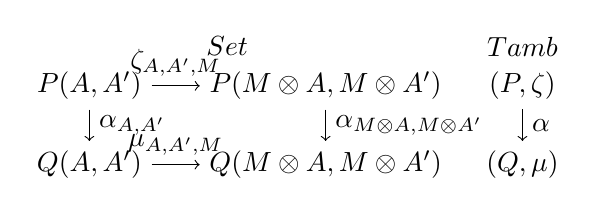
\begin{tikzpicture}[auto]
            \node (P) at (-1, 0) {$P(A,A')$};
            \node (Q) at (-1, -1) {$Q(A,A')$};
            \node (TP) at (2, 0) {$P(M\otimes A, M\otimes A')$};
            \node (TQ) at (2, -1) {$Q(M\otimes A, M\otimes A')$};
            \node (catpr) at (0.75, 0.5) {$\cat{Set}$};
  
            \draw[->] (P) to node{$\alpha_{A,A'}$}(Q);
            \draw[->] (P) to node{$\zeta_{A,A',M}$}(TP);
            \draw[->] (TP) to node{$\alpha_{M\otimes A,M\otimes A'}$}(TQ);
            \draw[->] (Q) to node{$\mu_{A,A',M}$}(TQ);
  
            \node (P) at (4.5, 0) {$(P,\zeta)$};
            \node (Q) at (4.5, -1) {$(Q,\mu)$};
            \draw[->] (P) to node{$\alpha$}(Q);
            \node (cattam) at (4.5, 0.5) {$\cat{Tamb}$};
  
          \end{tikzpicture}
          }
        \item[射の合成] 元の圏の射の合成からそのまま定義できる。
      \end{description}
      }
    \end{definition}
  \end{frame}
  \begin{frame}
    \frametitle{Opticの圏と丹原加群}
    \begin{theorem}
      \[\cat{Tamb}\simeq\incat{Optic}{Set}\]
    \end{theorem}
    ただし$\simeq$は左右の圏が圏同値であることを表している。また圏同値は圏の同型を緩めたものである。\\
    \vspace{\baselineskip}
    また$\incat{Optic}{Set}$は$\cat{Optic}$から$\cat{Set}$への準同型写像の成す圏である。  
  \end{frame}
  \begin{frame}
    
  \end{frame}
\end{document}